\documentclass[]{article}
\usepackage{lmodern}
\usepackage{amssymb,amsmath}
\usepackage{ifxetex,ifluatex}
\usepackage{fixltx2e} % provides \textsubscript
\ifnum 0\ifxetex 1\fi\ifluatex 1\fi=0 % if pdftex
  \usepackage[T1]{fontenc}
  \usepackage[utf8]{inputenc}
\else % if luatex or xelatex
  \ifxetex
    \usepackage{mathspec}
  \else
    \usepackage{fontspec}
  \fi
  \defaultfontfeatures{Ligatures=TeX,Scale=MatchLowercase}
\fi
% use upquote if available, for straight quotes in verbatim environments
\IfFileExists{upquote.sty}{\usepackage{upquote}}{}
% use microtype if available
\IfFileExists{microtype.sty}{%
\usepackage{microtype}
\UseMicrotypeSet[protrusion]{basicmath} % disable protrusion for tt fonts
}{}
\usepackage[margin=1in]{geometry}
\usepackage{hyperref}
\PassOptionsToPackage{usenames,dvipsnames}{color} % color is loaded by hyperref
\hypersetup{unicode=true,
            pdftitle={Week 2 - Homework},
            pdfauthor={STAT 420, Summer 2019, Josh Janda - joshlj2},
            colorlinks=true,
            linkcolor=Maroon,
            citecolor=Blue,
            urlcolor=cyan,
            breaklinks=true}
\urlstyle{same}  % don't use monospace font for urls
\usepackage{color}
\usepackage{fancyvrb}
\newcommand{\VerbBar}{|}
\newcommand{\VERB}{\Verb[commandchars=\\\{\}]}
\DefineVerbatimEnvironment{Highlighting}{Verbatim}{commandchars=\\\{\}}
% Add ',fontsize=\small' for more characters per line
\usepackage{framed}
\definecolor{shadecolor}{RGB}{248,248,248}
\newenvironment{Shaded}{\begin{snugshade}}{\end{snugshade}}
\newcommand{\KeywordTok}[1]{\textcolor[rgb]{0.13,0.29,0.53}{\textbf{#1}}}
\newcommand{\DataTypeTok}[1]{\textcolor[rgb]{0.13,0.29,0.53}{#1}}
\newcommand{\DecValTok}[1]{\textcolor[rgb]{0.00,0.00,0.81}{#1}}
\newcommand{\BaseNTok}[1]{\textcolor[rgb]{0.00,0.00,0.81}{#1}}
\newcommand{\FloatTok}[1]{\textcolor[rgb]{0.00,0.00,0.81}{#1}}
\newcommand{\ConstantTok}[1]{\textcolor[rgb]{0.00,0.00,0.00}{#1}}
\newcommand{\CharTok}[1]{\textcolor[rgb]{0.31,0.60,0.02}{#1}}
\newcommand{\SpecialCharTok}[1]{\textcolor[rgb]{0.00,0.00,0.00}{#1}}
\newcommand{\StringTok}[1]{\textcolor[rgb]{0.31,0.60,0.02}{#1}}
\newcommand{\VerbatimStringTok}[1]{\textcolor[rgb]{0.31,0.60,0.02}{#1}}
\newcommand{\SpecialStringTok}[1]{\textcolor[rgb]{0.31,0.60,0.02}{#1}}
\newcommand{\ImportTok}[1]{#1}
\newcommand{\CommentTok}[1]{\textcolor[rgb]{0.56,0.35,0.01}{\textit{#1}}}
\newcommand{\DocumentationTok}[1]{\textcolor[rgb]{0.56,0.35,0.01}{\textbf{\textit{#1}}}}
\newcommand{\AnnotationTok}[1]{\textcolor[rgb]{0.56,0.35,0.01}{\textbf{\textit{#1}}}}
\newcommand{\CommentVarTok}[1]{\textcolor[rgb]{0.56,0.35,0.01}{\textbf{\textit{#1}}}}
\newcommand{\OtherTok}[1]{\textcolor[rgb]{0.56,0.35,0.01}{#1}}
\newcommand{\FunctionTok}[1]{\textcolor[rgb]{0.00,0.00,0.00}{#1}}
\newcommand{\VariableTok}[1]{\textcolor[rgb]{0.00,0.00,0.00}{#1}}
\newcommand{\ControlFlowTok}[1]{\textcolor[rgb]{0.13,0.29,0.53}{\textbf{#1}}}
\newcommand{\OperatorTok}[1]{\textcolor[rgb]{0.81,0.36,0.00}{\textbf{#1}}}
\newcommand{\BuiltInTok}[1]{#1}
\newcommand{\ExtensionTok}[1]{#1}
\newcommand{\PreprocessorTok}[1]{\textcolor[rgb]{0.56,0.35,0.01}{\textit{#1}}}
\newcommand{\AttributeTok}[1]{\textcolor[rgb]{0.77,0.63,0.00}{#1}}
\newcommand{\RegionMarkerTok}[1]{#1}
\newcommand{\InformationTok}[1]{\textcolor[rgb]{0.56,0.35,0.01}{\textbf{\textit{#1}}}}
\newcommand{\WarningTok}[1]{\textcolor[rgb]{0.56,0.35,0.01}{\textbf{\textit{#1}}}}
\newcommand{\AlertTok}[1]{\textcolor[rgb]{0.94,0.16,0.16}{#1}}
\newcommand{\ErrorTok}[1]{\textcolor[rgb]{0.64,0.00,0.00}{\textbf{#1}}}
\newcommand{\NormalTok}[1]{#1}
\usepackage{longtable,booktabs}
\usepackage{graphicx,grffile}
\makeatletter
\def\maxwidth{\ifdim\Gin@nat@width>\linewidth\linewidth\else\Gin@nat@width\fi}
\def\maxheight{\ifdim\Gin@nat@height>\textheight\textheight\else\Gin@nat@height\fi}
\makeatother
% Scale images if necessary, so that they will not overflow the page
% margins by default, and it is still possible to overwrite the defaults
% using explicit options in \includegraphics[width, height, ...]{}
\setkeys{Gin}{width=\maxwidth,height=\maxheight,keepaspectratio}
\IfFileExists{parskip.sty}{%
\usepackage{parskip}
}{% else
\setlength{\parindent}{0pt}
\setlength{\parskip}{6pt plus 2pt minus 1pt}
}
\setlength{\emergencystretch}{3em}  % prevent overfull lines
\providecommand{\tightlist}{%
  \setlength{\itemsep}{0pt}\setlength{\parskip}{0pt}}
\setcounter{secnumdepth}{0}
% Redefines (sub)paragraphs to behave more like sections
\ifx\paragraph\undefined\else
\let\oldparagraph\paragraph
\renewcommand{\paragraph}[1]{\oldparagraph{#1}\mbox{}}
\fi
\ifx\subparagraph\undefined\else
\let\oldsubparagraph\subparagraph
\renewcommand{\subparagraph}[1]{\oldsubparagraph{#1}\mbox{}}
\fi

%%% Use protect on footnotes to avoid problems with footnotes in titles
\let\rmarkdownfootnote\footnote%
\def\footnote{\protect\rmarkdownfootnote}

%%% Change title format to be more compact
\usepackage{titling}

% Create subtitle command for use in maketitle
\providecommand{\subtitle}[1]{
  \posttitle{
    \begin{center}\large#1\end{center}
    }
}

\setlength{\droptitle}{-2em}

  \title{Week 2 - Homework}
    \pretitle{\vspace{\droptitle}\centering\huge}
  \posttitle{\par}
    \author{STAT 420, Summer 2019, Josh Janda - joshlj2}
    \preauthor{\centering\large\emph}
  \postauthor{\par}
    \date{}
    \predate{}\postdate{}
  

\begin{document}
\maketitle

\section{Directions}\label{directions}

\begin{itemize}
\tightlist
\item
  Be sure to remove this section if you use this \texttt{.Rmd} file as a
  template.
\item
  You may leave the questions in your final document.
\end{itemize}

\begin{center}\rule{0.5\linewidth}{\linethickness}\end{center}

\subsection{\texorpdfstring{Exercise 1 (Using
\texttt{lm})}{Exercise 1 (Using lm)}}\label{exercise-1-using-lm}

For this exercise we will use the \texttt{cats} dataset from the
\texttt{MASS} package. You should use \texttt{?cats} to learn about the
background of this dataset.

\textbf{(a)} Suppose we would like to understand the size of a cat's
heart based on the body weight of a cat. Fit a simple linear model in
\texttt{R} that accomplishes this task. Store the results in a variable
called \texttt{cat\_model}. Output the result of calling
\texttt{summary()} on \texttt{cat\_model}.

\begin{Shaded}
\begin{Highlighting}[]
\KeywordTok{library}\NormalTok{(MASS)}
\NormalTok{cat_model =}\StringTok{ }\KeywordTok{lm}\NormalTok{(Hwt }\OperatorTok{~}\StringTok{ }\NormalTok{Bwt, }\DataTypeTok{data=}\NormalTok{cats)}
\KeywordTok{summary}\NormalTok{(cat_model)}
\end{Highlighting}
\end{Shaded}

\begin{verbatim}
## 
## Call:
## lm(formula = Hwt ~ Bwt, data = cats)
## 
## Residuals:
##     Min      1Q  Median      3Q     Max 
## -3.5694 -0.9634 -0.0921  1.0426  5.1238 
## 
## Coefficients:
##             Estimate Std. Error t value Pr(>|t|)    
## (Intercept)  -0.3567     0.6923  -0.515    0.607    
## Bwt           4.0341     0.2503  16.119   <2e-16 ***
## ---
## Signif. codes:  0 '***' 0.001 '**' 0.01 '*' 0.05 '.' 0.1 ' ' 1
## 
## Residual standard error: 1.452 on 142 degrees of freedom
## Multiple R-squared:  0.6466, Adjusted R-squared:  0.6441 
## F-statistic: 259.8 on 1 and 142 DF,  p-value: < 2.2e-16
\end{verbatim}

\textbf{(b)} Output only the estimated regression coefficients.
Interpret \(\hat{\beta_0}\) and \(\beta_1\) in the \emph{context of the
problem}. Be aware that only one of those is an estimate.

\begin{Shaded}
\begin{Highlighting}[]
\NormalTok{cat_model}\OperatorTok{$}\NormalTok{coefficients}
\end{Highlighting}
\end{Shaded}

\begin{verbatim}
## (Intercept)         Bwt 
##  -0.3566624   4.0340627
\end{verbatim}

\(\hat{\beta_0}\) is the intercept of the model and can be interpreted
as the size of a cat's heart if the body weight of a cat is zero. In
numerical terms, if a cat's body weight is equal to zero then we would
predict it's heart size to be -.3567. \(\beta_1\) is the true population
slope coefficient, so in the population it means that the size of a cats
heart increases by \(\beta_1\) with a one unit increase in body weight.
We do not know the true \(\beta_1\), so we must estimate it using our
sample data.

\textbf{(c)} Use your model to predict the heart weight of a cat that
weights \textbf{2.7} kg. Do you feel confident in this prediction?
Briefly explain.

\begin{Shaded}
\begin{Highlighting}[]
\NormalTok{predict_c =}\StringTok{ }\KeywordTok{data.frame}\NormalTok{(}\DataTypeTok{Bwt =} \KeywordTok{c}\NormalTok{(}\FloatTok{2.7}\NormalTok{))}
\KeywordTok{predict}\NormalTok{(cat_model, }\DataTypeTok{newdata =}\NormalTok{ predict_c)}
\end{Highlighting}
\end{Shaded}

\begin{verbatim}
##        1 
## 10.53531
\end{verbatim}

\begin{Shaded}
\begin{Highlighting}[]
\NormalTok{cats}\OperatorTok{$}\NormalTok{Bwt}
\end{Highlighting}
\end{Shaded}

\begin{verbatim}
##   [1] 2.0 2.0 2.0 2.1 2.1 2.1 2.1 2.1 2.1 2.1 2.1 2.1 2.2 2.2 2.2 2.2 2.2
##  [18] 2.2 2.3 2.3 2.3 2.3 2.3 2.3 2.3 2.3 2.3 2.3 2.3 2.3 2.4 2.4 2.4 2.4
##  [35] 2.5 2.5 2.6 2.6 2.6 2.7 2.7 2.7 2.9 2.9 2.9 3.0 3.0 2.0 2.0 2.1 2.2
##  [52] 2.2 2.2 2.2 2.2 2.2 2.2 2.2 2.3 2.4 2.4 2.4 2.4 2.4 2.5 2.5 2.5 2.5
##  [69] 2.5 2.5 2.5 2.5 2.6 2.6 2.6 2.6 2.6 2.6 2.7 2.7 2.7 2.7 2.7 2.7 2.7
##  [86] 2.7 2.7 2.8 2.8 2.8 2.8 2.8 2.8 2.8 2.9 2.9 2.9 2.9 2.9 3.0 3.0 3.0
## [103] 3.0 3.0 3.0 3.0 3.0 3.0 3.1 3.1 3.1 3.1 3.1 3.1 3.2 3.2 3.2 3.2 3.2
## [120] 3.2 3.3 3.3 3.3 3.3 3.3 3.4 3.4 3.4 3.4 3.4 3.5 3.5 3.5 3.5 3.5 3.6
## [137] 3.6 3.6 3.6 3.7 3.8 3.8 3.9 3.9
\end{verbatim}

I feel confident in this prediction due to our dataset containing values
either exactly 2.7 or close to 2.7 kg. Since our dataset contains this
value, it will be able to more accurately predict the heart weight.

\textbf{(d)} Use your model to predict the heart weight of a cat that
weights \textbf{4.4} kg. Do you feel confident in this prediction?
Briefly explain.

\begin{Shaded}
\begin{Highlighting}[]
\NormalTok{predict_d =}\StringTok{ }\KeywordTok{data.frame}\NormalTok{(}\DataTypeTok{Bwt =} \KeywordTok{c}\NormalTok{(}\FloatTok{4.4}\NormalTok{))}
\KeywordTok{predict}\NormalTok{(cat_model, }\DataTypeTok{newdata =}\NormalTok{ predict_d)}
\end{Highlighting}
\end{Shaded}

\begin{verbatim}
##        1 
## 17.39321
\end{verbatim}

I do not feel confident in this prediction since our dataset does not
contain any values greater than 3.9. This will make this prediction
inaccurate and therefore unreliable and I cannot be confident in it's
predicted value.

\textbf{(e)} Create a scatterplot of the data and add the fitted
regression line. Make sure your plot is well labeled and is somewhat
visually appealing.

\begin{Shaded}
\begin{Highlighting}[]
\KeywordTok{library}\NormalTok{(ggplot2)}
\end{Highlighting}
\end{Shaded}

\begin{verbatim}
## Warning: package 'ggplot2' was built under R version 3.5.2
\end{verbatim}

\begin{Shaded}
\begin{Highlighting}[]
\KeywordTok{ggplot}\NormalTok{(cats, }\KeywordTok{aes}\NormalTok{(}\DataTypeTok{x =}\NormalTok{ Bwt, }\DataTypeTok{y =}\NormalTok{ Hwt)) }\OperatorTok{+}\StringTok{ }\KeywordTok{geom_point}\NormalTok{(}\KeywordTok{aes}\NormalTok{(}\DataTypeTok{size =}\NormalTok{ Bwt), }\DataTypeTok{color =} \StringTok{'cyan'}\NormalTok{) }\OperatorTok{+}\StringTok{ }\KeywordTok{ggtitle}\NormalTok{(}\StringTok{'Heart Size vs Body Weight in Cats'}\NormalTok{) }\OperatorTok{+}\StringTok{ }\KeywordTok{xlab}\NormalTok{(}\StringTok{'Body Weight (Kg)'}\NormalTok{) }\OperatorTok{+}\StringTok{ }\KeywordTok{ylab}\NormalTok{(}\StringTok{'Heart Size'}\NormalTok{) }\OperatorTok{+}\StringTok{ }\KeywordTok{theme}\NormalTok{(}\DataTypeTok{plot.title =} \KeywordTok{element_text}\NormalTok{(}\DataTypeTok{hjust=}\NormalTok{.}\DecValTok{5}\NormalTok{)) }\OperatorTok{+}\StringTok{ }\KeywordTok{geom_smooth}\NormalTok{(}\DataTypeTok{method =}\NormalTok{ lm, }\DataTypeTok{formula =}\NormalTok{ y }\OperatorTok{~}\StringTok{ }\NormalTok{x, }\KeywordTok{aes}\NormalTok{(}\DataTypeTok{color =} \StringTok{'yellow'}\NormalTok{)) }\OperatorTok{+}\StringTok{ }\KeywordTok{scale_color_manual}\NormalTok{(}\DataTypeTok{values =} \KeywordTok{c}\NormalTok{(}\StringTok{'yellow'}\NormalTok{), }\DataTypeTok{labels=}\KeywordTok{c}\NormalTok{(}\StringTok{'Fitted Regression Line'}\NormalTok{), }\DataTypeTok{name =} \StringTok{'Legend'}\NormalTok{)}
\end{Highlighting}
\end{Shaded}

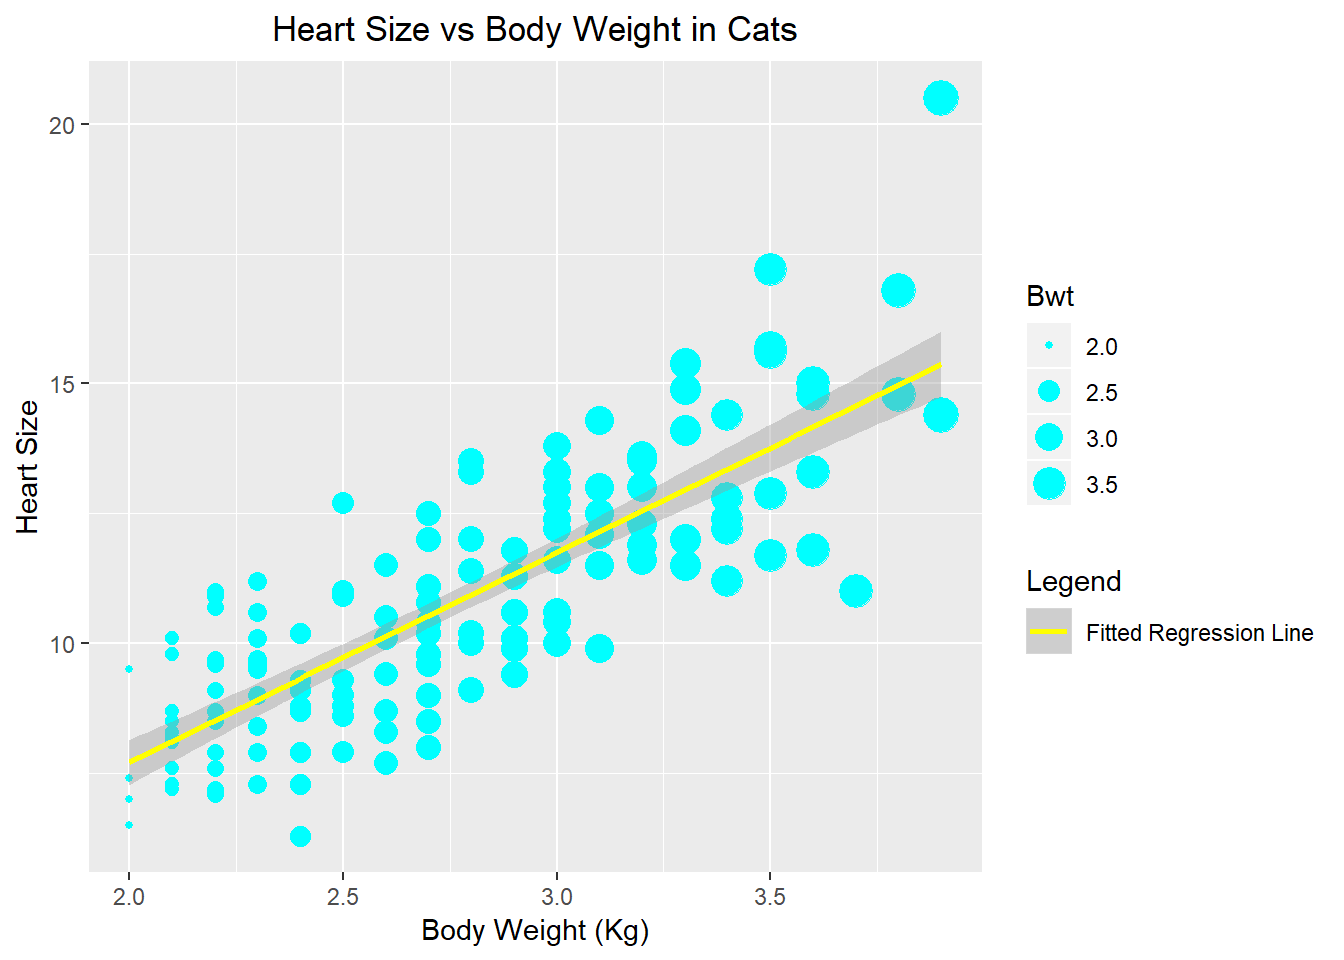
\includegraphics{w02-hw-joshlj2_files/figure-latex/unnamed-chunk-5-1.pdf}

\textbf{(f)} Report the value of \(R^2\) for the model. Do so directly.
Do not simply copy and paste the value from the full output in the
console after running \texttt{summary()} in part \textbf{(a)}.

\begin{Shaded}
\begin{Highlighting}[]
\CommentTok{#summary(cat_model)$r.squared Do not use summary..}
\NormalTok{SSR_q1 =}\StringTok{ }\KeywordTok{sum}\NormalTok{(}\KeywordTok{resid}\NormalTok{(cat_model)}\OperatorTok{^}\DecValTok{2}\NormalTok{)}
\NormalTok{SST_q1 =}\StringTok{ }\KeywordTok{sum}\NormalTok{((cats}\OperatorTok{$}\NormalTok{Hwt }\OperatorTok{-}\StringTok{ }\KeywordTok{mean}\NormalTok{(cats}\OperatorTok{$}\NormalTok{Hwt))}\OperatorTok{^}\DecValTok{2}\NormalTok{)}
\DecValTok{1} \OperatorTok{-}\StringTok{ }\NormalTok{(SSR_q1 }\OperatorTok{/}\StringTok{ }\NormalTok{SST_q1)}
\end{Highlighting}
\end{Shaded}

\begin{verbatim}
## [1] 0.6466209
\end{verbatim}

\begin{Shaded}
\begin{Highlighting}[]
\CommentTok{#or}
\KeywordTok{summary}\NormalTok{(cat_model)}\OperatorTok{$}\NormalTok{r.squared}
\end{Highlighting}
\end{Shaded}

\begin{verbatim}
## [1] 0.6466209
\end{verbatim}

\begin{center}\rule{0.5\linewidth}{\linethickness}\end{center}

\subsection{Exercise 2 (Writing
Functions)}\label{exercise-2-writing-functions}

This exercise is a continuation of Exercise 1.

\textbf{(a)} Write a function called \texttt{get\_sd\_est} that
calculates an estimate of \(\sigma\) in one of two ways depending on
input to the function. The function should take three arguments as
input:

\begin{itemize}
\tightlist
\item
  \texttt{fitted\_vals} - A vector of fitted values from a model
\item
  \texttt{actual\_vals} - A vector of the true values of the response
\item
  \texttt{mle} - A logical (\texttt{TRUE} / \texttt{FALSE}) variable
  which defaults to \texttt{FALSE}
\end{itemize}

The function should return a single value:

\begin{itemize}
\tightlist
\item
  \(s_e\) if \texttt{mle} is set to \texttt{FALSE}.
\item
  \(\hat{\sigma}\) if \texttt{mle} is set to \texttt{TRUE}.
\end{itemize}

\begin{Shaded}
\begin{Highlighting}[]
\NormalTok{get_sd_est =}\StringTok{ }\ControlFlowTok{function}\NormalTok{(fitted_vals, actual_vals, }\DataTypeTok{mle =} \OtherTok{FALSE}\NormalTok{) \{}
\NormalTok{  residuals_func =}\StringTok{ }\NormalTok{actual_vals }\OperatorTok{-}\StringTok{ }\NormalTok{fitted_vals}
\NormalTok{  RSS =}\StringTok{ }\KeywordTok{sum}\NormalTok{(residuals_func}\OperatorTok{^}\DecValTok{2}\NormalTok{)}
  \ControlFlowTok{if}\NormalTok{ (mle }\OperatorTok{==}\StringTok{ }\OtherTok{TRUE}\NormalTok{) \{}
    \KeywordTok{sqrt}\NormalTok{(RSS }\OperatorTok{/}\StringTok{ }\KeywordTok{length}\NormalTok{(residuals_func))}
\NormalTok{  \}}\ControlFlowTok{else}\NormalTok{\{}
    \KeywordTok{sqrt}\NormalTok{(RSS }\OperatorTok{/}\StringTok{ }\NormalTok{(}\KeywordTok{length}\NormalTok{(residuals_func) }\OperatorTok{-}\StringTok{ }\DecValTok{2}\NormalTok{))}
\NormalTok{  \}}
\NormalTok{\}}
\end{Highlighting}
\end{Shaded}

\textbf{(b)} Run the function \texttt{get\_sd\_est} on the residuals
from the model in Exercise 1, with \texttt{mle} set to \texttt{FALSE}.
Explain the resulting estimate in the context of the model.

\begin{Shaded}
\begin{Highlighting}[]
\KeywordTok{get_sd_est}\NormalTok{(cat_model}\OperatorTok{$}\NormalTok{fitted.values, cats}\OperatorTok{$}\NormalTok{Hwt, }\DataTypeTok{mle =} \OtherTok{FALSE}\NormalTok{)}
\end{Highlighting}
\end{Shaded}

\begin{verbatim}
## [1] 1.452373
\end{verbatim}

This estimate is with mle set to false. The estimate we get is with
adjustments to the number of parameters in the model, which is two. We
do this since we are building our model from sample data, not a
population. Since this is typically how standard error of regression is
calculated, this estimate will match the estimate we get from our model
summary. We also do this calculation since we do not know the true
\({\sigma}\), so we must estimate it using this calculation which gives
\(s_e\).

\textbf{(c)} Run the function \texttt{get\_sd\_est} on the residuals
from the model in Exercise 1, with \texttt{mle} set to \texttt{TRUE}.
Explain the resulting estimate in the context of the model. Note that we
are trying to estimate the same parameter as in part \textbf{(b)}.

\begin{Shaded}
\begin{Highlighting}[]
\KeywordTok{get_sd_est}\NormalTok{(cat_model}\OperatorTok{$}\NormalTok{fitted, cats}\OperatorTok{$}\NormalTok{Hwt, }\DataTypeTok{mle=}\OtherTok{TRUE}\NormalTok{)}
\end{Highlighting}
\end{Shaded}

\begin{verbatim}
## [1] 1.442252
\end{verbatim}

With mle set to true, we are trying to estimate population parameters.
In this case, we do not adjust for degrees of freedom (number of
parameters in the model). This will give us the estimated value of
\({\sigma}\) and not the standard error of regression (\(s_e\)).

\textbf{(d)} To check your work, output
\texttt{summary(cat\_model)\$sigma}. It should match at least one of
\textbf{(b)} or \textbf{(c)}.

\begin{Shaded}
\begin{Highlighting}[]
\KeywordTok{summary}\NormalTok{(cat_model)}\OperatorTok{$}\NormalTok{sigma}
\end{Highlighting}
\end{Shaded}

\begin{verbatim}
## [1] 1.452373
\end{verbatim}

Matches part b, which is consistent with my reasoning in part b.

\begin{center}\rule{0.5\linewidth}{\linethickness}\end{center}

\subsection{Exercise 3 (Simulating
SLR)}\label{exercise-3-simulating-slr}

Consider the model

\[
Y_i = 5 + -3 x_i + \epsilon_i
\]

with

\[
\epsilon_i \sim N(\mu = 0, \sigma^2 = 10.24)
\]

where \(\beta_0 = 5\) and \(\beta_1 = -3\).

This exercise relies heavily on generating random observations. To make
this reproducible we will set a seed for the randomization. Alter the
following code to make \texttt{birthday} store your birthday in the
format: \texttt{yyyymmdd}. For example,
\href{https://en.wikipedia.org/wiki/William_Sealy_Gosset}{William
Gosset}, better known as \emph{Student}, was born on June 13, 1876, so
he would use:

\begin{Shaded}
\begin{Highlighting}[]
\NormalTok{birthday =}\StringTok{ }\DecValTok{19981127}
\KeywordTok{set.seed}\NormalTok{(birthday)}
\end{Highlighting}
\end{Shaded}

\textbf{(a)} Use \texttt{R} to simulate \texttt{n\ =\ 25} observations
from the above model. For the remainder of this exercise, use the
following ``known'' values of \(x\).

\begin{Shaded}
\begin{Highlighting}[]
\NormalTok{x =}\StringTok{ }\KeywordTok{runif}\NormalTok{(}\DataTypeTok{n =} \DecValTok{25}\NormalTok{, }\DecValTok{0}\NormalTok{, }\DecValTok{10}\NormalTok{)}
\end{Highlighting}
\end{Shaded}

You may use
\href{http://daviddalpiaz.github.io/appliedstats/simple-linear-regression.html\#simulating-slr}{the
\texttt{sim\_slr} function provided in the text}. Store the data frame
this function returns in a variable of your choice. Note that this
function calls \(y\) \texttt{response} and \(x\) \texttt{predictor}.

\begin{Shaded}
\begin{Highlighting}[]
\NormalTok{sim_slr =}\StringTok{ }\ControlFlowTok{function}\NormalTok{(x, beta_}\DecValTok{0}\NormalTok{, beta_}\DecValTok{1}\NormalTok{, sigma_squared) \{}
\NormalTok{  n =}\StringTok{ }\KeywordTok{length}\NormalTok{(x)}
\NormalTok{  epsilon =}\StringTok{ }\KeywordTok{rnorm}\NormalTok{(n, }\DataTypeTok{mean=}\DecValTok{0}\NormalTok{, }\DataTypeTok{sd =} \KeywordTok{sqrt}\NormalTok{(sigma_squared))}
\NormalTok{  y =}\StringTok{ }\NormalTok{beta_}\DecValTok{0} \OperatorTok{+}\StringTok{ }\NormalTok{beta_}\DecValTok{1}\OperatorTok{*}\NormalTok{x }\OperatorTok{+}\StringTok{ }\NormalTok{epsilon}
  \KeywordTok{data.frame}\NormalTok{(}\DataTypeTok{predictor =}\NormalTok{ x, }\DataTypeTok{response =}\NormalTok{ y)}
\NormalTok{\}}
\NormalTok{sim_data_q3 =}\StringTok{ }\KeywordTok{sim_slr}\NormalTok{(x, }\DataTypeTok{beta_0 =} \DecValTok{5}\NormalTok{, }\DataTypeTok{beta_1 =} \OperatorTok{-}\DecValTok{3}\NormalTok{, }\DataTypeTok{sigma_squared =} \FloatTok{10.24}\NormalTok{)}
\end{Highlighting}
\end{Shaded}

\textbf{(b)} Fit a model to your simulated data. Report the estimated
coefficients. Are they close to what you would expect? Briefly explain.

\begin{Shaded}
\begin{Highlighting}[]
\NormalTok{fitted_model_q3 =}\StringTok{ }\KeywordTok{lm}\NormalTok{(sim_data_q3}\OperatorTok{$}\NormalTok{response }\OperatorTok{~}\StringTok{ }\NormalTok{sim_data_q3}\OperatorTok{$}\NormalTok{predictor)}
\NormalTok{fitted_model_q3}\OperatorTok{$}\NormalTok{coefficients}
\end{Highlighting}
\end{Shaded}

\begin{verbatim}
##           (Intercept) sim_data_q3$predictor 
##              4.915486             -3.005269
\end{verbatim}

\textbf{(c)} Plot the data you simulated in part \textbf{(a)}. Add the
regression line from part \textbf{(b)} as well as the line for the true
model. Hint: Keep all plotting commands in the same chunk.

\begin{Shaded}
\begin{Highlighting}[]
\KeywordTok{library}\NormalTok{(ggplot2)}
\KeywordTok{ggplot}\NormalTok{(sim_data_q3, }\KeywordTok{aes}\NormalTok{(}\DataTypeTok{x=}\NormalTok{predictor, }\DataTypeTok{y=}\NormalTok{response)) }\OperatorTok{+}\StringTok{ }\KeywordTok{geom_point}\NormalTok{(}\DataTypeTok{color=}\StringTok{'limegreen'}\NormalTok{) }\OperatorTok{+}\StringTok{ }\KeywordTok{geom_smooth}\NormalTok{(}\DataTypeTok{method=}\StringTok{'lm'}\NormalTok{, }\DataTypeTok{formula =}\NormalTok{ y}\OperatorTok{~}\NormalTok{x, }\KeywordTok{aes}\NormalTok{(}\DataTypeTok{color =} \StringTok{"deeppink"}\NormalTok{), }\DataTypeTok{se=}\OtherTok{FALSE}\NormalTok{, }\DataTypeTok{show.legend =} \OtherTok{TRUE}\NormalTok{) }\OperatorTok{+}\StringTok{ }\KeywordTok{geom_abline}\NormalTok{(}\KeywordTok{aes}\NormalTok{(}\DataTypeTok{slope =} \OperatorTok{-}\DecValTok{3}\NormalTok{, }\DataTypeTok{intercept =} \DecValTok{5}\NormalTok{, }\DataTypeTok{color=}\StringTok{"orange"}\NormalTok{), }\DataTypeTok{show.legend =} \OtherTok{TRUE}\NormalTok{) }\OperatorTok{+}\StringTok{ }\KeywordTok{labs}\NormalTok{(}\DataTypeTok{x =} \StringTok{"Predictor"}\NormalTok{, }\DataTypeTok{y =} \StringTok{"Response"}\NormalTok{) }\OperatorTok{+}\StringTok{ }\KeywordTok{scale_color_manual}\NormalTok{(}\DataTypeTok{name =} \StringTok{"Key"}\NormalTok{, }\DataTypeTok{values =} \KeywordTok{c}\NormalTok{(}\StringTok{"deeppink"}\NormalTok{, }\StringTok{"orange"}\NormalTok{), }\DataTypeTok{labels =} \KeywordTok{c}\NormalTok{(}\StringTok{"Estimated Regression Line"}\NormalTok{, }\StringTok{"Actual Line"}\NormalTok{)) }\OperatorTok{+}\StringTok{ }\KeywordTok{ggtitle}\NormalTok{(}\StringTok{"Response vs Predictor"}\NormalTok{) }\OperatorTok{+}\StringTok{ }\KeywordTok{theme}\NormalTok{(}\DataTypeTok{plot.title =} \KeywordTok{element_text}\NormalTok{(}\DataTypeTok{hjust=}\NormalTok{.}\DecValTok{5}\NormalTok{))}
\end{Highlighting}
\end{Shaded}

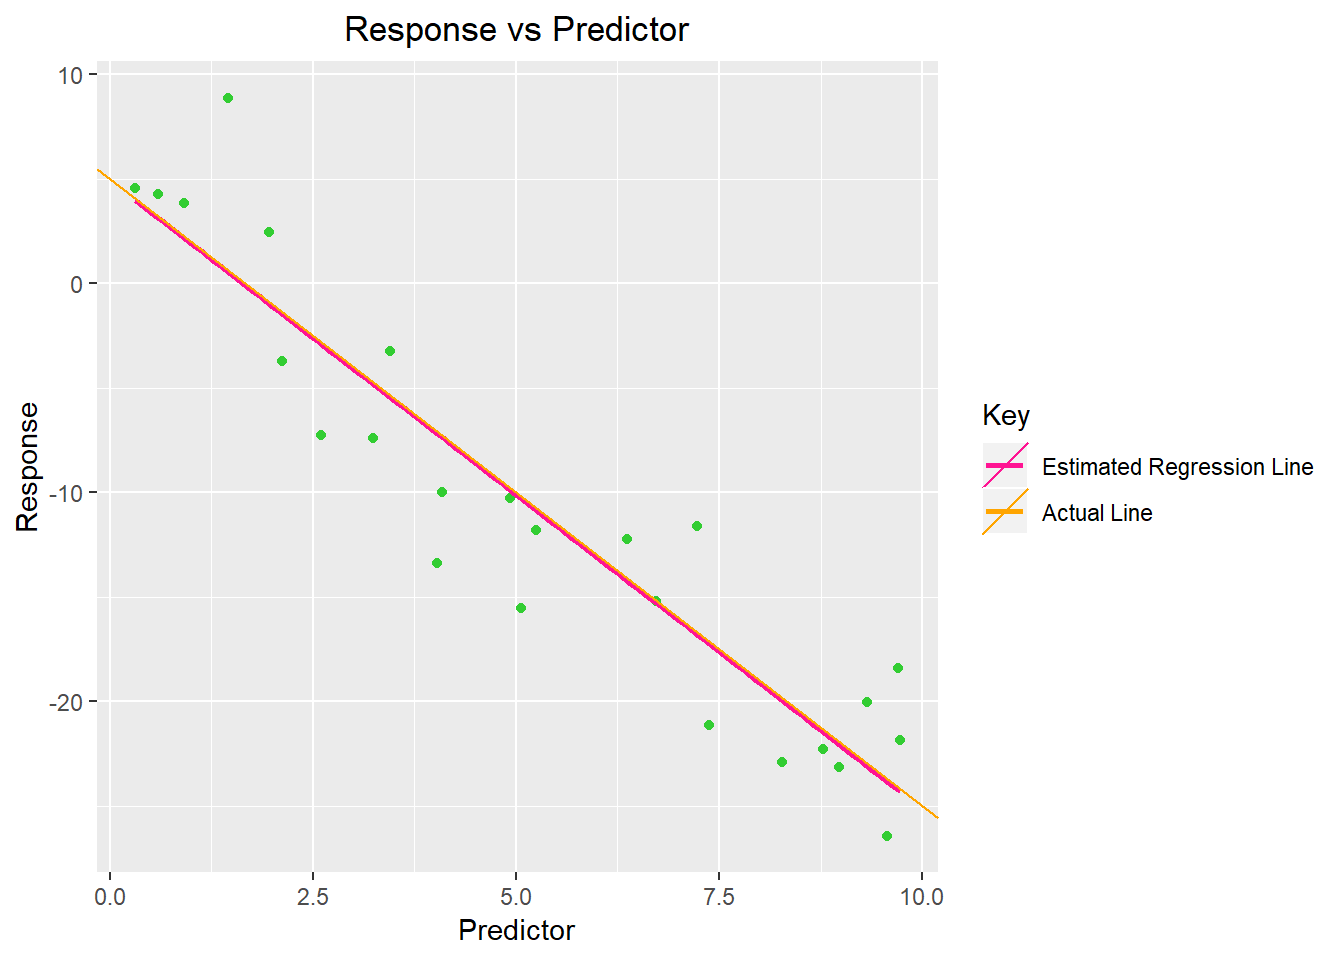
\includegraphics{w02-hw-joshlj2_files/figure-latex/unnamed-chunk-15-1.pdf}

\textbf{(d)} Use \texttt{R} to repeat the process of simulating
\texttt{n\ =\ 25} observations from the above model \(1500\) times. Each
time fit a SLR model to the data and store the value of
\(\hat{\beta_1}\) in a variable called \texttt{beta\_hat\_1}. Some
hints:

\begin{itemize}
\tightlist
\item
  Consider a \texttt{for} loop.
\item
  Create \texttt{beta\_hat\_1} before writing the \texttt{for} loop.
  Make it a vector of length \(1500\) where each element is \texttt{0}.
\item
  Inside the body of the \texttt{for} loop, simulate new \(y\) data each
  time. Use a variable to temporarily store this data together with the
  known \(x\) data as a data frame.
\item
  After simulating the data, use \texttt{lm()} to fit a regression. Use
  a variable to temporarily store this output.
\item
  Use the \texttt{coef()} function and \texttt{{[}{]}} to extract the
  correct estimated coefficient.
\item
  Use \texttt{beta\_hat\_1{[}i{]}} to store in elements of
  \texttt{beta\_hat\_1}.
\item
  See the notes on
  \href{http://daviddalpiaz.github.io/appliedstats/introduction-to-r.html\#distribution-of-a-sample-mean}{Distribution
  of a Sample Mean} for some inspiration.
\end{itemize}

You can do this differently if you like. Use of these hints is not
required.

\begin{Shaded}
\begin{Highlighting}[]
\NormalTok{beta_hat_}\DecValTok{1}\NormalTok{ =}\StringTok{ }\KeywordTok{rep}\NormalTok{(}\DecValTok{0}\NormalTok{, }\DecValTok{1500}\NormalTok{)}
\ControlFlowTok{for}\NormalTok{ (i }\ControlFlowTok{in} \DecValTok{1}\OperatorTok{:}\KeywordTok{length}\NormalTok{(beta_hat_}\DecValTok{1}\NormalTok{)}\OperatorTok{-}\DecValTok{1}\NormalTok{) \{}
\NormalTok{  temp_data =}\StringTok{ }\KeywordTok{sim_slr}\NormalTok{(x, }\DataTypeTok{beta_0 =} \DecValTok{5}\NormalTok{, }\DataTypeTok{beta_1 =} \OperatorTok{-}\DecValTok{3}\NormalTok{, }\DataTypeTok{sigma_squared =} \FloatTok{10.24}\NormalTok{)}
\NormalTok{  temp_model =}\StringTok{ }\KeywordTok{lm}\NormalTok{(temp_data}\OperatorTok{$}\NormalTok{response }\OperatorTok{~}\StringTok{ }\NormalTok{temp_data}\OperatorTok{$}\NormalTok{predictor)}
  
\NormalTok{  beta_hat_}\DecValTok{1}\NormalTok{[i] =}\StringTok{ }\NormalTok{temp_model}\OperatorTok{$}\NormalTok{coefficients[[}\DecValTok{2}\NormalTok{]]}
\NormalTok{\}}
\CommentTok{#look at distribution of beta_hat_1.. should be approx normal with mean -3.}
\CommentTok{#hist(beta_hat_1, breaks=60)}
\end{Highlighting}
\end{Shaded}

\textbf{(e)} Report the mean and standard deviation of
\texttt{beta\_hat\_1}. Do either of these look familiar?

\begin{Shaded}
\begin{Highlighting}[]
\KeywordTok{mean}\NormalTok{(beta_hat_}\DecValTok{1}\NormalTok{)}
\end{Highlighting}
\end{Shaded}

\begin{verbatim}
## [1] -2.994451
\end{verbatim}

\begin{Shaded}
\begin{Highlighting}[]
\KeywordTok{sd}\NormalTok{(beta_hat_}\DecValTok{1}\NormalTok{)}
\end{Highlighting}
\end{Shaded}

\begin{verbatim}
## [1] 0.2188817
\end{verbatim}

The mean of \(\hat{\beta}_1\) looks familiar, as it is the true value of
\(\beta_1\). Since we simulated the value of \(\hat{\beta}_1\) 1,500
times the list of values should have a mean very close to the true value
of \(\beta_1\), as long as our estimates are unbiased. The standard
deviation of \(\hat{\beta}_1\) looks familiar as well, and should be
very close to the standard error of \(\hat{\beta}_1\), which looking at
the summary of the original model we made confirms this. See below:

\begin{Shaded}
\begin{Highlighting}[]
\KeywordTok{summary}\NormalTok{(fitted_model_q3)}\OperatorTok{$}\NormalTok{coefficients[}\DecValTok{2}\NormalTok{,}\DecValTok{2}\NormalTok{]}
\end{Highlighting}
\end{Shaded}

\begin{verbatim}
## [1] 0.2362496
\end{verbatim}

\textbf{(f)} Plot a histogram of \texttt{beta\_hat\_1}. Comment on the
shape of this histogram.

\begin{Shaded}
\begin{Highlighting}[]
\NormalTok{beta_hat_1_df =}\StringTok{ }\KeywordTok{data.frame}\NormalTok{(}\DataTypeTok{betahat1 =}\NormalTok{ beta_hat_}\DecValTok{1}\NormalTok{)}
\KeywordTok{ggplot}\NormalTok{(beta_hat_1_df, }\KeywordTok{aes}\NormalTok{(}\DataTypeTok{x=}\NormalTok{betahat1)) }\OperatorTok{+}\StringTok{ }\KeywordTok{geom_histogram}\NormalTok{(}\KeywordTok{aes}\NormalTok{(}\DataTypeTok{fill=}\StringTok{'orange'}\NormalTok{), }\DataTypeTok{bins =} \DecValTok{60}\NormalTok{) }\OperatorTok{+}\StringTok{ }\KeywordTok{xlab}\NormalTok{(}\StringTok{'Beta Hat 1 Values'}\NormalTok{) }\OperatorTok{+}\StringTok{ }\KeywordTok{ggtitle}\NormalTok{(}\StringTok{'Histogram of Beta Hat 1'}\NormalTok{) }\OperatorTok{+}\StringTok{ }\KeywordTok{theme}\NormalTok{(}\DataTypeTok{plot.title =} \KeywordTok{element_text}\NormalTok{(}\DataTypeTok{hjust =} \FloatTok{0.5}\NormalTok{))}
\end{Highlighting}
\end{Shaded}

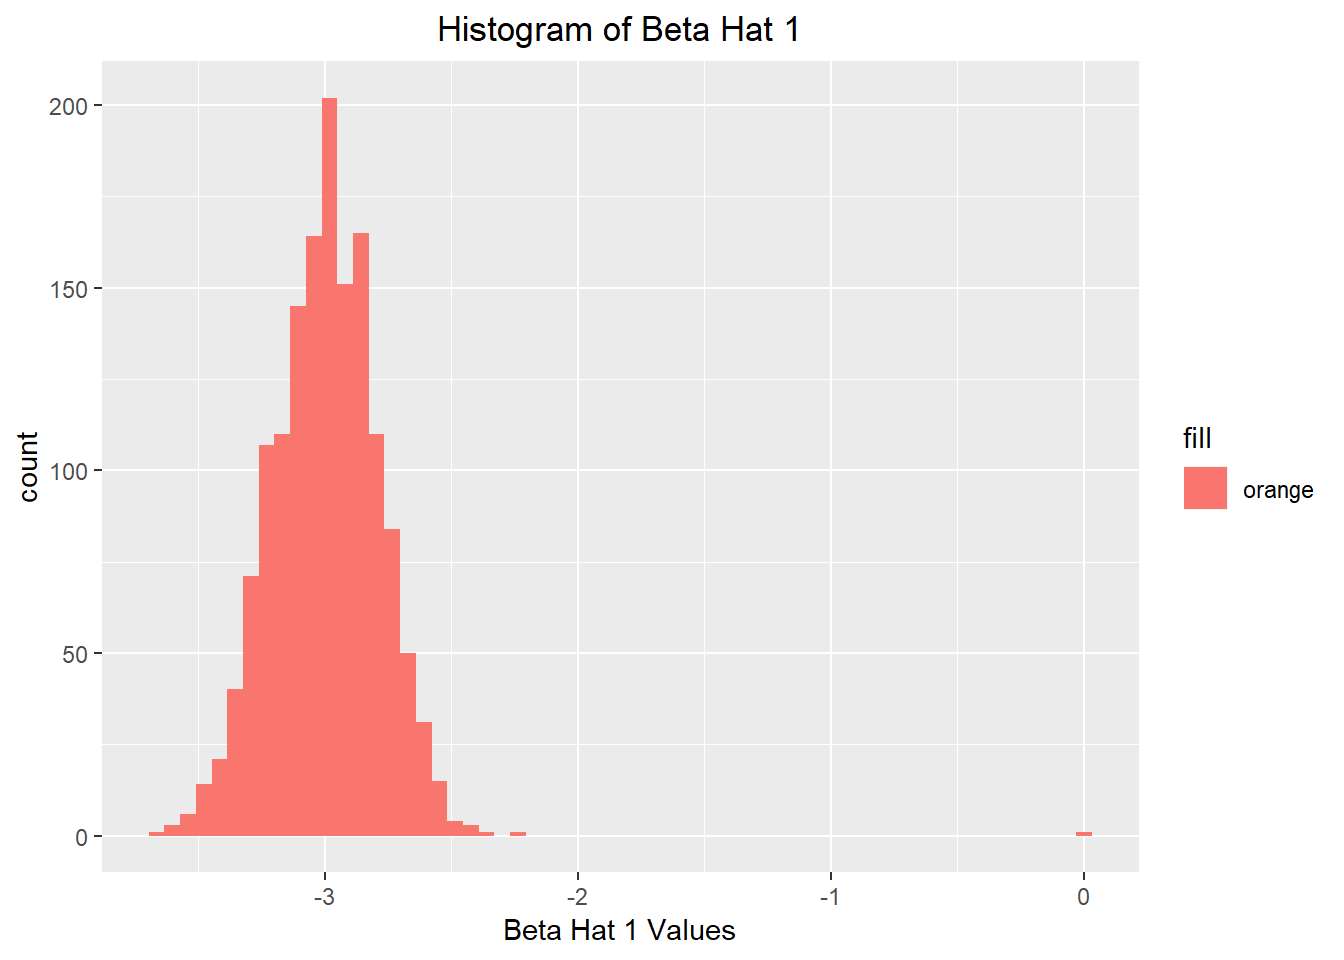
\includegraphics{w02-hw-joshlj2_files/figure-latex/unnamed-chunk-19-1.pdf}
The shape of the histogram is as expected. The distribution of
\(\hat{\beta}_1\), when simulated 1,500 times, is centered (mean) around
-3, which is the coefficient of beta one. The distribution is also very
close to normal, which confirms the central limit theorem. The more beta
hat ones you simulate, the more the histogram collapses into center -3.
This is shown below:

\begin{Shaded}
\begin{Highlighting}[]
\NormalTok{beta_hat_1_extra =}\StringTok{ }\KeywordTok{rep}\NormalTok{(}\DecValTok{0}\NormalTok{, }\DecValTok{10000}\NormalTok{)}
\ControlFlowTok{for}\NormalTok{ (i }\ControlFlowTok{in} \DecValTok{1}\OperatorTok{:}\KeywordTok{length}\NormalTok{(beta_hat_1_extra)}\OperatorTok{-}\DecValTok{1}\NormalTok{) \{}
\NormalTok{  temp_data =}\StringTok{ }\KeywordTok{sim_slr}\NormalTok{(x, }\DataTypeTok{beta_0 =} \DecValTok{5}\NormalTok{, }\DataTypeTok{beta_1 =} \OperatorTok{-}\DecValTok{3}\NormalTok{, }\DataTypeTok{sigma_squared =} \FloatTok{10.24}\NormalTok{)}
\NormalTok{  temp_model =}\StringTok{ }\KeywordTok{lm}\NormalTok{(temp_data}\OperatorTok{$}\NormalTok{response }\OperatorTok{~}\StringTok{ }\NormalTok{temp_data}\OperatorTok{$}\NormalTok{predictor)}
  
\NormalTok{  beta_hat_1_extra[i] =}\StringTok{ }\NormalTok{temp_model}\OperatorTok{$}\NormalTok{coefficients[[}\DecValTok{2}\NormalTok{]]}
\NormalTok{\}}

\NormalTok{beta_hat_1_extradf =}\StringTok{ }\KeywordTok{data.frame}\NormalTok{(}\DataTypeTok{betahat1 =}\NormalTok{ beta_hat_1_extra)}
\KeywordTok{ggplot}\NormalTok{(beta_hat_1_extradf, }\KeywordTok{aes}\NormalTok{(}\DataTypeTok{x=}\NormalTok{betahat1)) }\OperatorTok{+}\StringTok{ }\KeywordTok{geom_histogram}\NormalTok{(}\KeywordTok{aes}\NormalTok{(}\DataTypeTok{fill=}\StringTok{'orange'}\NormalTok{), }\DataTypeTok{bins =} \DecValTok{60}\NormalTok{) }\OperatorTok{+}\StringTok{ }\KeywordTok{xlab}\NormalTok{(}\StringTok{'Beta Hat 1 Values'}\NormalTok{) }\OperatorTok{+}\StringTok{ }\KeywordTok{ggtitle}\NormalTok{(}\StringTok{'Histogram of Beta Hat 1'}\NormalTok{) }\OperatorTok{+}\StringTok{ }\KeywordTok{theme}\NormalTok{(}\DataTypeTok{plot.title =} \KeywordTok{element_text}\NormalTok{(}\DataTypeTok{hjust =} \FloatTok{0.5}\NormalTok{))}
\end{Highlighting}
\end{Shaded}

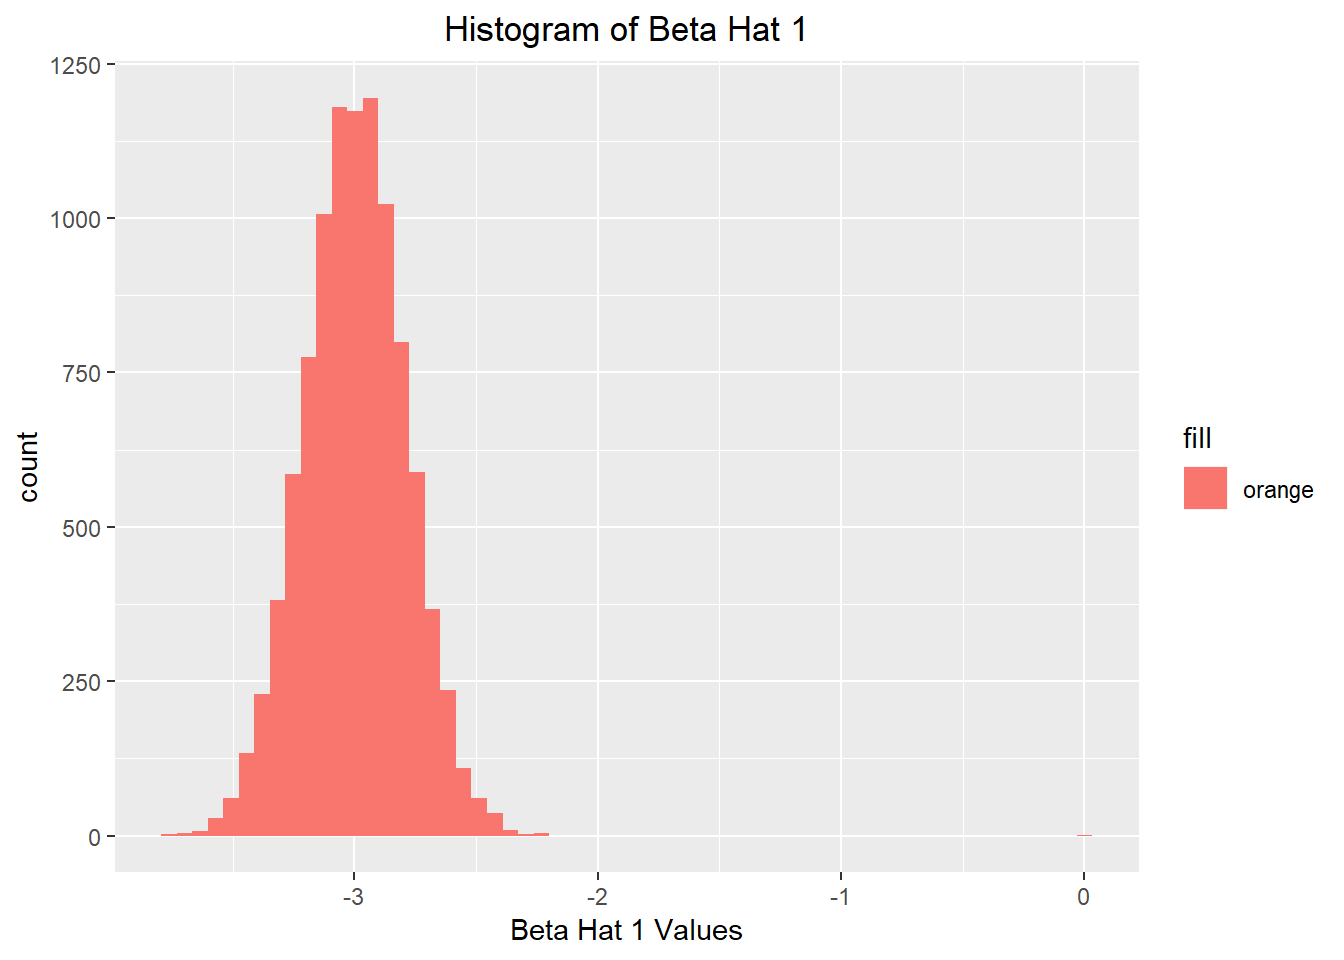
\includegraphics{w02-hw-joshlj2_files/figure-latex/unnamed-chunk-20-1.pdf}

\begin{center}\rule{0.5\linewidth}{\linethickness}\end{center}

\subsection{Exercise 4 (Be a Skeptic)}\label{exercise-4-be-a-skeptic}

Consider the model

\[
Y_i = 3 + 0 \cdot x_i + \epsilon_i
\]

with

\[
\epsilon_i \sim N(\mu = 0, \sigma^2 = 4)
\]

where \(\beta_0 = 3\) and \(\beta_1 = 0\).

Before answering the following parts, set a seed value equal to
\textbf{your} birthday, as was done in the previous exercise.

\begin{Shaded}
\begin{Highlighting}[]
\NormalTok{birthday =}\StringTok{ }\DecValTok{19981127}
\KeywordTok{set.seed}\NormalTok{(birthday)}
\end{Highlighting}
\end{Shaded}

\textbf{(a)} Use \texttt{R} to repeat the process of simulating
\texttt{n\ =\ 75} observations from the above model \(2500\) times. For
the remainder of this exercise, use the following ``known'' values of
\(x\).

\begin{Shaded}
\begin{Highlighting}[]
\NormalTok{x =}\StringTok{ }\KeywordTok{runif}\NormalTok{(}\DataTypeTok{n =} \DecValTok{75}\NormalTok{, }\DecValTok{0}\NormalTok{, }\DecValTok{10}\NormalTok{)}
\NormalTok{beta_hat_}\DecValTok{1}\NormalTok{ =}\StringTok{ }\KeywordTok{rep}\NormalTok{(}\DecValTok{0}\NormalTok{, }\DecValTok{2500}\NormalTok{)}
\ControlFlowTok{for}\NormalTok{ (i }\ControlFlowTok{in} \DecValTok{1}\OperatorTok{:}\KeywordTok{length}\NormalTok{(beta_hat_}\DecValTok{1}\NormalTok{)}\OperatorTok{-}\DecValTok{1}\NormalTok{) \{}
\NormalTok{  temp_data =}\StringTok{ }\KeywordTok{sim_slr}\NormalTok{(x, }\DataTypeTok{beta_0 =} \DecValTok{3}\NormalTok{, }\DataTypeTok{beta_1 =} \DecValTok{0}\NormalTok{, }\DataTypeTok{sigma_squared =} \DecValTok{4}\NormalTok{)}
\NormalTok{  temp_model =}\StringTok{ }\KeywordTok{lm}\NormalTok{(temp_data}\OperatorTok{$}\NormalTok{response }\OperatorTok{~}\StringTok{ }\NormalTok{temp_data}\OperatorTok{$}\NormalTok{predictor)}
  
\NormalTok{  beta_hat_}\DecValTok{1}\NormalTok{[i] =}\StringTok{ }\NormalTok{temp_model}\OperatorTok{$}\NormalTok{coefficients[[}\DecValTok{2}\NormalTok{]]}
\NormalTok{\}}
\end{Highlighting}
\end{Shaded}

Each time fit a SLR model to the data and store the value of
\(\hat{\beta_1}\) in a variable called \texttt{beta\_hat\_1}. You may
use
\href{http://daviddalpiaz.github.io/appliedstats/simple-linear-regression.html\#simulating-slr}{the
\texttt{sim\_slr} function provided in the text}. Hint: Yes
\(\beta_1 = 0\).

\textbf{(b)} Plot a histogram of \texttt{beta\_hat\_1}. Comment on the
shape of this histogram.

\begin{Shaded}
\begin{Highlighting}[]
\NormalTok{beta_hat_1_df =}\StringTok{ }\KeywordTok{data.frame}\NormalTok{(}\DataTypeTok{betahat1 =}\NormalTok{ beta_hat_}\DecValTok{1}\NormalTok{)}
\KeywordTok{ggplot}\NormalTok{(beta_hat_1_df, }\KeywordTok{aes}\NormalTok{(}\DataTypeTok{x=}\NormalTok{betahat1)) }\OperatorTok{+}\StringTok{ }\KeywordTok{geom_histogram}\NormalTok{(}\KeywordTok{aes}\NormalTok{(}\DataTypeTok{fill=}\StringTok{'orange'}\NormalTok{), }\DataTypeTok{bins =} \DecValTok{60}\NormalTok{) }\OperatorTok{+}\StringTok{ }\KeywordTok{xlab}\NormalTok{(}\StringTok{'Beta Hat 1 Values'}\NormalTok{) }\OperatorTok{+}\StringTok{ }\KeywordTok{ggtitle}\NormalTok{(}\StringTok{'Histogram of Beta Hat 1'}\NormalTok{) }\OperatorTok{+}\StringTok{ }\KeywordTok{theme}\NormalTok{(}\DataTypeTok{plot.title =} \KeywordTok{element_text}\NormalTok{(}\DataTypeTok{hjust =} \FloatTok{0.5}\NormalTok{))}
\end{Highlighting}
\end{Shaded}

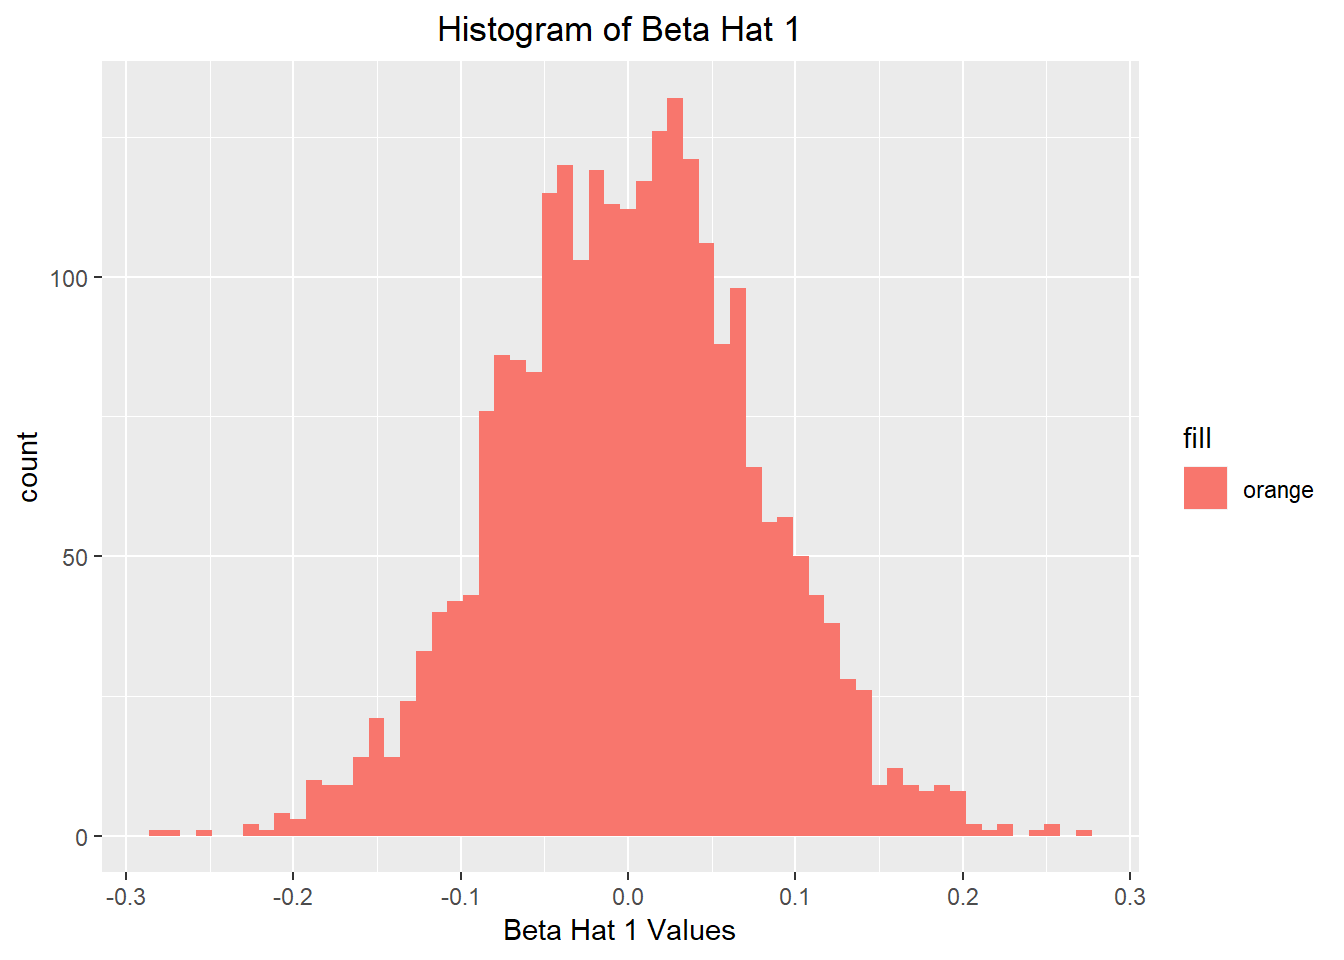
\includegraphics{w02-hw-joshlj2_files/figure-latex/unnamed-chunk-23-1.pdf}

\textbf{(c)} Import the data in \href{skeptic.csv}{\texttt{skeptic.csv}}
and fit a SLR model. The variable names in \texttt{skeptic.csv} follow
the same convention as those returned by \texttt{sim\_slr()}. Extract
the fitted coefficient for \(\beta_1\).

\begin{Shaded}
\begin{Highlighting}[]
\KeywordTok{library}\NormalTok{(readr)}
\end{Highlighting}
\end{Shaded}

\begin{verbatim}
## Warning: package 'readr' was built under R version 3.5.2
\end{verbatim}

\begin{Shaded}
\begin{Highlighting}[]
\NormalTok{skeptic =}\StringTok{ }\KeywordTok{read.csv}\NormalTok{(}\StringTok{'skeptic.csv'}\NormalTok{)}
\NormalTok{skeptic_mod =}\StringTok{ }\KeywordTok{lm}\NormalTok{(skeptic}\OperatorTok{$}\NormalTok{response }\OperatorTok{~}\StringTok{ }\NormalTok{skeptic}\OperatorTok{$}\NormalTok{predictor)}
\NormalTok{skeptic_beta1 =}\StringTok{ }\NormalTok{skeptic_mod}\OperatorTok{$}\NormalTok{coefficients[[}\DecValTok{2}\NormalTok{]]}
\end{Highlighting}
\end{Shaded}

\textbf{(d)} Re-plot the histogram from \textbf{(b)}. Now add a vertical
red line at the value of \(\hat{\beta_1}\) in part \textbf{(c)}. To do
so, you'll need to use \texttt{abline(v\ =\ c,\ col\ =\ "red")} where
\texttt{c} is your value.

\begin{Shaded}
\begin{Highlighting}[]
\KeywordTok{ggplot}\NormalTok{(beta_hat_1_df, }\KeywordTok{aes}\NormalTok{(}\DataTypeTok{x=}\NormalTok{betahat1)) }\OperatorTok{+}\StringTok{ }\KeywordTok{geom_histogram}\NormalTok{(}\KeywordTok{aes}\NormalTok{(}\DataTypeTok{fill=}\StringTok{'orange'}\NormalTok{), }\DataTypeTok{bins =} \DecValTok{60}\NormalTok{) }\OperatorTok{+}\StringTok{ }\KeywordTok{geom_vline}\NormalTok{(}\DataTypeTok{xintercept =}\NormalTok{ skeptic_beta1, }\DataTypeTok{col=}\StringTok{'blue'}\NormalTok{)}
\end{Highlighting}
\end{Shaded}

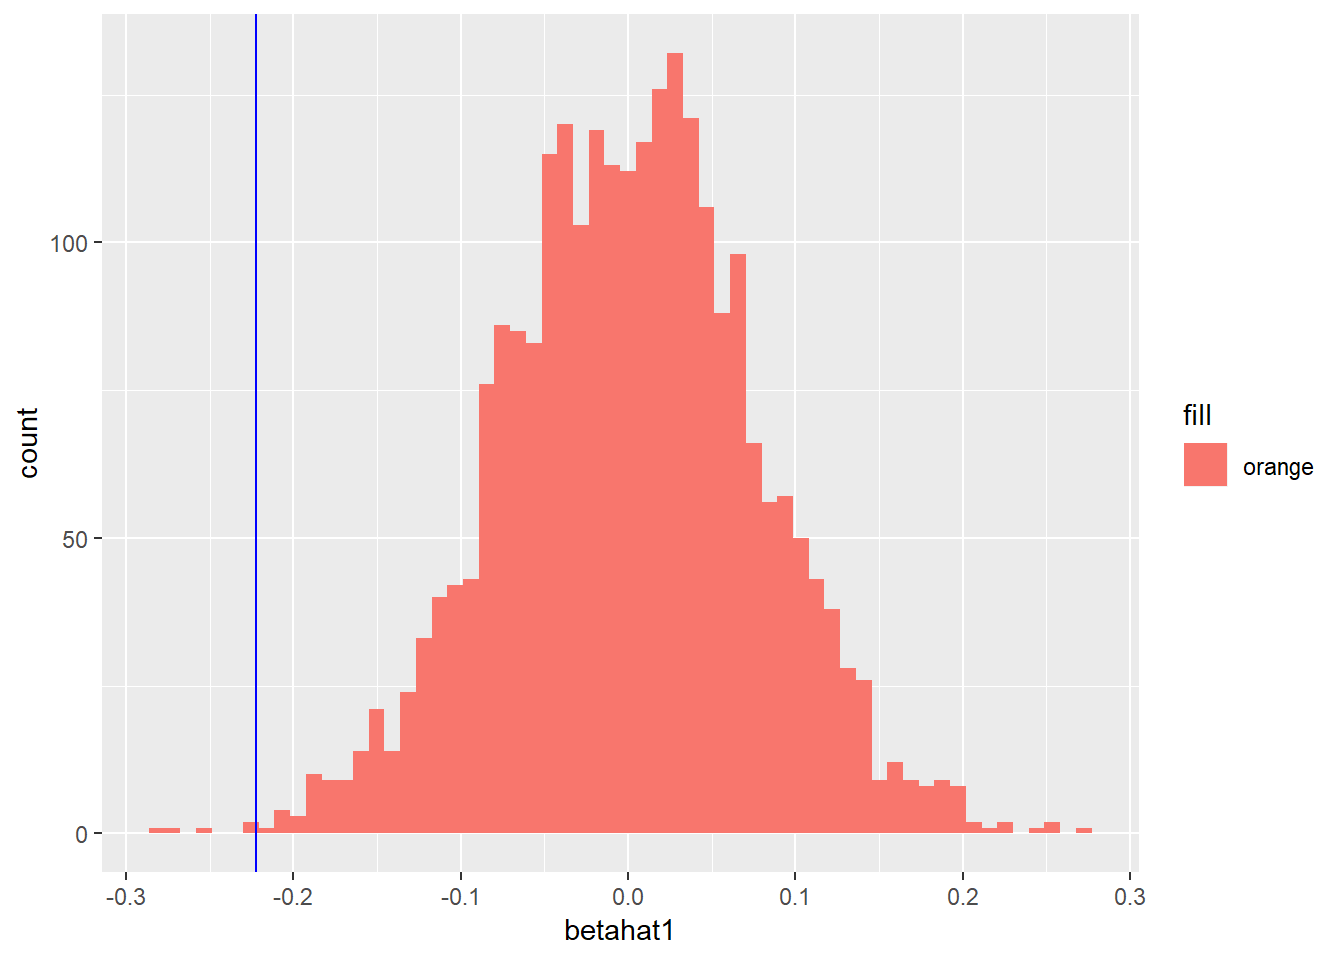
\includegraphics{w02-hw-joshlj2_files/figure-latex/unnamed-chunk-25-1.pdf}

\textbf{(e)} Your value of \(\hat{\beta_1}\) in \textbf{(c)} should be
negative. What proportion of the \texttt{beta\_hat\_1} values is smaller
than your \(\hat{\beta_1}\)? Return this proportion, as well as this
proportion multiplied by \texttt{2}.

\begin{Shaded}
\begin{Highlighting}[]
\KeywordTok{length}\NormalTok{(beta_hat_}\DecValTok{1}\NormalTok{[}\KeywordTok{which}\NormalTok{(beta_hat_}\DecValTok{1} \OperatorTok{<}\StringTok{ }\NormalTok{skeptic_beta1)]) }\OperatorTok{/}\StringTok{ }\KeywordTok{length}\NormalTok{(beta_hat_}\DecValTok{1}\NormalTok{)}
\end{Highlighting}
\end{Shaded}

\begin{verbatim}
## [1] 0.0016
\end{verbatim}

\begin{Shaded}
\begin{Highlighting}[]
\KeywordTok{length}\NormalTok{(beta_hat_}\DecValTok{1}\NormalTok{[}\KeywordTok{which}\NormalTok{(beta_hat_}\DecValTok{1} \OperatorTok{<}\StringTok{ }\NormalTok{skeptic_beta1)]) }\OperatorTok{/}\StringTok{ }\KeywordTok{length}\NormalTok{(beta_hat_}\DecValTok{1}\NormalTok{) }\OperatorTok{*}\StringTok{ }\DecValTok{2}
\end{Highlighting}
\end{Shaded}

\begin{verbatim}
## [1] 0.0032
\end{verbatim}

\textbf{(f)} Based on your histogram and part \textbf{(e)}, do you think
the \href{skeptic.csv}{\texttt{s\ \ keptic.csv}} data could have been
generated by the model given above? Briefly explain. I believe that
there is a small chance that the skeptic data could have been generated
by the model given above. There is a just a very small chance that it
could have happened, but there is a non-zero probability as shown above
by the proportions. Since the skeptic data is only one set of 75 points,
and we generated 2500 sets, it is definitely possible since some of our
generated datasets has a beta hat 1 less than the skeptic datasets beta
hat 1.

\begin{center}\rule{0.5\linewidth}{\linethickness}\end{center}

\subsection{Exercise 5 (Comparing
Models)}\label{exercise-5-comparing-models}

For this exercise we will use the \texttt{Ozone} dataset from the
\texttt{mlbench} package. You should use \texttt{?Ozone} to learn about
the background of this dataset. You may need to install the
\texttt{mlbench} package. If you do so, do not include code to install
the package in your \texttt{R} Markdown document.

For simplicity, we will perform some data cleaning before proceeding.

\begin{Shaded}
\begin{Highlighting}[]
\KeywordTok{data}\NormalTok{(Ozone, }\DataTypeTok{package =} \StringTok{"mlbench"}\NormalTok{)}
\NormalTok{Ozone =}\StringTok{ }\NormalTok{Ozone[, }\KeywordTok{c}\NormalTok{(}\DecValTok{4}\NormalTok{, }\DecValTok{6}\NormalTok{, }\DecValTok{7}\NormalTok{, }\DecValTok{8}\NormalTok{)]}
\KeywordTok{colnames}\NormalTok{(Ozone) =}\StringTok{ }\KeywordTok{c}\NormalTok{(}\StringTok{"ozone"}\NormalTok{, }\StringTok{"wind"}\NormalTok{, }\StringTok{"humidity"}\NormalTok{, }\StringTok{"temp"}\NormalTok{)}
\NormalTok{Ozone =}\StringTok{ }\NormalTok{Ozone[}\KeywordTok{complete.cases}\NormalTok{(Ozone), ]}
\end{Highlighting}
\end{Shaded}

We have:

\begin{itemize}
\tightlist
\item
  Loaded the data from the package
\item
  Subset the data to relevant variables

  \begin{itemize}
  \tightlist
  \item
    This is not really necessary (or perhaps a good idea) but it makes
    the next step easier
  \end{itemize}
\item
  Given variables useful names
\item
  Removed any observation with missing values

  \begin{itemize}
  \tightlist
  \item
    This should be given much more thought in practice
  \end{itemize}
\end{itemize}

For this exercise we will define the ``Root Mean Square Error'' of a
model as

\[
\text{RMSE} = \sqrt{\frac{1}{n} \sum_{i = 1}^{n}(y_i - \hat{y}_i)^2}.
\]

\textbf{(a)} Fit three SLR models, each with ``ozone'' as the response.
For the predictor, use ``wind speed,'' ``humidity percentage,'' and
``temperature'' respectively. For each, calculate \(\text{RMSE}\) and
\(R^2\). Arrange the results in a markdown table, with a row for each
model. Suggestion: Create a data frame that stores the results, then
investigate the \texttt{kable()} function from the \texttt{knitr}
package.

\begin{Shaded}
\begin{Highlighting}[]
\KeywordTok{library}\NormalTok{(forecast)}\CommentTok{#use forecasting library to obtain accuracy function..}
\end{Highlighting}
\end{Shaded}

\begin{verbatim}
## Warning: package 'forecast' was built under R version 3.5.2
\end{verbatim}

\begin{Shaded}
\begin{Highlighting}[]
\KeywordTok{library}\NormalTok{(knitr)}
\NormalTok{q5_model1 =}\StringTok{ }\KeywordTok{lm}\NormalTok{(Ozone}\OperatorTok{$}\NormalTok{ozone }\OperatorTok{~}\StringTok{ }\NormalTok{Ozone}\OperatorTok{$}\NormalTok{wind)}
\NormalTok{q5_model2 =}\StringTok{ }\KeywordTok{lm}\NormalTok{(Ozone}\OperatorTok{$}\NormalTok{ozone }\OperatorTok{~}\StringTok{ }\NormalTok{Ozone}\OperatorTok{$}\NormalTok{humidity)}
\NormalTok{q5_model3 =}\StringTok{ }\KeywordTok{lm}\NormalTok{(Ozone}\OperatorTok{$}\NormalTok{ozone }\OperatorTok{~}\StringTok{ }\NormalTok{Ozone}\OperatorTok{$}\NormalTok{temp)}


\NormalTok{results =}\StringTok{ }\KeywordTok{data.frame}\NormalTok{(}\DataTypeTok{model1 =} \KeywordTok{c}\NormalTok{(}\DataTypeTok{model_rmse =} \KeywordTok{data.frame}\NormalTok{(}\KeywordTok{accuracy}\NormalTok{(q5_model1))}\OperatorTok{$}\NormalTok{RMSE, }\DataTypeTok{model_r2 =} \KeywordTok{summary}\NormalTok{(q5_model1)}\OperatorTok{$}\NormalTok{r.squared),}
                     \DataTypeTok{model2 =} \KeywordTok{c}\NormalTok{(}\DataTypeTok{model2rmse =} \KeywordTok{data.frame}\NormalTok{(}\KeywordTok{accuracy}\NormalTok{(q5_model2))}\OperatorTok{$}\NormalTok{RMSE, }\DataTypeTok{model2r2 =} \KeywordTok{summary}\NormalTok{(q5_model2)}\OperatorTok{$}\NormalTok{r.squared),}
                     \DataTypeTok{model3 =} \KeywordTok{c}\NormalTok{(}\DataTypeTok{model3rmse =} \KeywordTok{data.frame}\NormalTok{(}\KeywordTok{accuracy}\NormalTok{(q5_model3))}\OperatorTok{$}\NormalTok{RMSE, }\DataTypeTok{model3r2 =} \KeywordTok{summary}\NormalTok{(q5_model3)}\OperatorTok{$}\NormalTok{r.squared)}
\NormalTok{)}

\KeywordTok{kable}\NormalTok{(}\KeywordTok{head}\NormalTok{(}\KeywordTok{t}\NormalTok{(results)))}
\end{Highlighting}
\end{Shaded}

\begin{longtable}[]{@{}lrr@{}}
\toprule
& model\_rmse & model\_r2\tabularnewline
\midrule
\endhead
model1 & 7.961695 & 0.0001402\tabularnewline
model2 & 7.147822 & 0.1941105\tabularnewline
model3 & 5.009257 & 0.6042011\tabularnewline
\bottomrule
\end{longtable}

\textbf{(b)} Based on the results, which of the three predictors used is
most helpful for predicting ozone readings? Briefly explain.

Based on the results, the third model with temperature as the predictor
is the most helpful for predicting ozone readings. This model has the
lowest Root Mean Square Error, and the highest R-Squared. This model
explains the data the best out of all three.

\begin{center}\rule{0.5\linewidth}{\linethickness}\end{center}

\subsection{Exercise 00 (SLR without
Intercept)}\label{exercise-00-slr-without-intercept}

\textbf{This exercise will \emph{not} be graded and is simply provided
for your information. No credit will be given for the completion of this
exercise. Give it a try now, and be sure to read the solutions later.}

Sometimes it can be reasonable to assume that \(\beta_0\) should be 0.
That is, the line should pass through the point \((0, 0)\). For example,
if a car is traveling 0 miles per hour, its stopping distance should be
0! (Unlike what we saw in the book.)

We can simply define a model without an intercept,

\[
Y_i = \beta x_i + \epsilon_i.
\]

\textbf{(a)}
\href{http://daviddalpiaz.github.io/appliedstats/simple-linear-regression.html\#least-squares-approach}{In
the \textbf{Least Squares Approach} section of the text} you saw the
calculus behind the derivation of the regression estimates, and then we
performed the calculation for the \texttt{cars} dataset using
\texttt{R}. Here you need to do, but not show, the derivation for the
slope only model. You should then use that derivation of \(\hat{\beta}\)
to write a function that performs the calculation for the estimate you
derived.

In summary, use the method of least squares to derive an estimate for
\(\beta\) using data points \((x_i, y_i)\) for \(i = 1, 2, \ldots n\).
Simply put, find the value of \(\beta\) to minimize the function

\[
f(\beta)=\sum_{i=1}^{n}(y_{i}-\beta x_{i})^{2}.
\]

Then, write a function \texttt{get\_beta\_no\_int} that takes input:

\begin{itemize}
\tightlist
\item
  \texttt{x} - A predictor variable
\item
  \texttt{y} - A response variable
\end{itemize}

The function should then output the \(\hat{\beta}\) you derived for a
given set of data.

\textbf{(b)} Write your derivation in your \texttt{.Rmd} file using TeX.
Or write your derivation by hand, scan or photograph your work, and
insert it into the \texttt{.Rmd} as an image. See the
\href{http://rmarkdown.rstudio.com/}{RMarkdown documentation} for
working with images.

\textbf{(c)} Test your function on the \texttt{cats} data using body
weight as \texttt{x} and heart weight as \texttt{y}. What is the
estimate for \(\beta\) for this data?

\textbf{(d)} Check your work in \texttt{R}. The following syntax can be
used to fit a model without an intercept:

\begin{Shaded}
\begin{Highlighting}[]
\KeywordTok{lm}\NormalTok{(response }\OperatorTok{~}\StringTok{ }\DecValTok{0} \OperatorTok{+}\StringTok{ }\NormalTok{predictor, }\DataTypeTok{data =}\NormalTok{ dataset)}
\end{Highlighting}
\end{Shaded}

Use this to fit a model to the \texttt{cat} data without an intercept.
Output the coefficient of the fitted model. It should match your answer
to \textbf{(c)}.


\end{document}
